% Generated by Sphinx.
\def\sphinxdocclass{report}
\documentclass[letterpaper,10pt,english]{sphinxmanual}
\usepackage[utf8]{inputenc}
\DeclareUnicodeCharacter{00A0}{\nobreakspace}
\usepackage[T1]{fontenc}
\usepackage{babel}
\usepackage{times}
\usepackage[Bjarne]{fncychap}
\usepackage{longtable}
\usepackage{sphinx}
\usepackage{multirow}


\title{HIPSR Documentation}
\date{October 30, 2012}
\release{1.0}
\author{Danny Price}
\newcommand{\sphinxlogo}{}
\renewcommand{\releasename}{Release}
\makeindex

\makeatletter
\def\PYG@reset{\let\PYG@it=\relax \let\PYG@bf=\relax%
    \let\PYG@ul=\relax \let\PYG@tc=\relax%
    \let\PYG@bc=\relax \let\PYG@ff=\relax}
\def\PYG@tok#1{\csname PYG@tok@#1\endcsname}
\def\PYG@toks#1+{\ifx\relax#1\empty\else%
    \PYG@tok{#1}\expandafter\PYG@toks\fi}
\def\PYG@do#1{\PYG@bc{\PYG@tc{\PYG@ul{%
    \PYG@it{\PYG@bf{\PYG@ff{#1}}}}}}}
\def\PYG#1#2{\PYG@reset\PYG@toks#1+\relax+\PYG@do{#2}}

\def\PYG@tok@gd{\def\PYG@tc##1{\textcolor[rgb]{0.63,0.00,0.00}{##1}}}
\def\PYG@tok@gu{\let\PYG@bf=\textbf\def\PYG@tc##1{\textcolor[rgb]{0.50,0.00,0.50}{##1}}}
\def\PYG@tok@gt{\def\PYG@tc##1{\textcolor[rgb]{0.00,0.25,0.82}{##1}}}
\def\PYG@tok@gs{\let\PYG@bf=\textbf}
\def\PYG@tok@gr{\def\PYG@tc##1{\textcolor[rgb]{1.00,0.00,0.00}{##1}}}
\def\PYG@tok@cm{\let\PYG@it=\textit\def\PYG@tc##1{\textcolor[rgb]{0.25,0.50,0.56}{##1}}}
\def\PYG@tok@vg{\def\PYG@tc##1{\textcolor[rgb]{0.73,0.38,0.84}{##1}}}
\def\PYG@tok@m{\def\PYG@tc##1{\textcolor[rgb]{0.13,0.50,0.31}{##1}}}
\def\PYG@tok@mh{\def\PYG@tc##1{\textcolor[rgb]{0.13,0.50,0.31}{##1}}}
\def\PYG@tok@cs{\def\PYG@tc##1{\textcolor[rgb]{0.25,0.50,0.56}{##1}}\def\PYG@bc##1{\colorbox[rgb]{1.00,0.94,0.94}{##1}}}
\def\PYG@tok@ge{\let\PYG@it=\textit}
\def\PYG@tok@vc{\def\PYG@tc##1{\textcolor[rgb]{0.73,0.38,0.84}{##1}}}
\def\PYG@tok@il{\def\PYG@tc##1{\textcolor[rgb]{0.13,0.50,0.31}{##1}}}
\def\PYG@tok@go{\def\PYG@tc##1{\textcolor[rgb]{0.19,0.19,0.19}{##1}}}
\def\PYG@tok@cp{\def\PYG@tc##1{\textcolor[rgb]{0.00,0.44,0.13}{##1}}}
\def\PYG@tok@gi{\def\PYG@tc##1{\textcolor[rgb]{0.00,0.63,0.00}{##1}}}
\def\PYG@tok@gh{\let\PYG@bf=\textbf\def\PYG@tc##1{\textcolor[rgb]{0.00,0.00,0.50}{##1}}}
\def\PYG@tok@ni{\let\PYG@bf=\textbf\def\PYG@tc##1{\textcolor[rgb]{0.84,0.33,0.22}{##1}}}
\def\PYG@tok@nl{\let\PYG@bf=\textbf\def\PYG@tc##1{\textcolor[rgb]{0.00,0.13,0.44}{##1}}}
\def\PYG@tok@nn{\let\PYG@bf=\textbf\def\PYG@tc##1{\textcolor[rgb]{0.05,0.52,0.71}{##1}}}
\def\PYG@tok@no{\def\PYG@tc##1{\textcolor[rgb]{0.38,0.68,0.84}{##1}}}
\def\PYG@tok@na{\def\PYG@tc##1{\textcolor[rgb]{0.25,0.44,0.63}{##1}}}
\def\PYG@tok@nb{\def\PYG@tc##1{\textcolor[rgb]{0.00,0.44,0.13}{##1}}}
\def\PYG@tok@nc{\let\PYG@bf=\textbf\def\PYG@tc##1{\textcolor[rgb]{0.05,0.52,0.71}{##1}}}
\def\PYG@tok@nd{\let\PYG@bf=\textbf\def\PYG@tc##1{\textcolor[rgb]{0.33,0.33,0.33}{##1}}}
\def\PYG@tok@ne{\def\PYG@tc##1{\textcolor[rgb]{0.00,0.44,0.13}{##1}}}
\def\PYG@tok@nf{\def\PYG@tc##1{\textcolor[rgb]{0.02,0.16,0.49}{##1}}}
\def\PYG@tok@si{\let\PYG@it=\textit\def\PYG@tc##1{\textcolor[rgb]{0.44,0.63,0.82}{##1}}}
\def\PYG@tok@s2{\def\PYG@tc##1{\textcolor[rgb]{0.25,0.44,0.63}{##1}}}
\def\PYG@tok@vi{\def\PYG@tc##1{\textcolor[rgb]{0.73,0.38,0.84}{##1}}}
\def\PYG@tok@nt{\let\PYG@bf=\textbf\def\PYG@tc##1{\textcolor[rgb]{0.02,0.16,0.45}{##1}}}
\def\PYG@tok@nv{\def\PYG@tc##1{\textcolor[rgb]{0.73,0.38,0.84}{##1}}}
\def\PYG@tok@s1{\def\PYG@tc##1{\textcolor[rgb]{0.25,0.44,0.63}{##1}}}
\def\PYG@tok@gp{\let\PYG@bf=\textbf\def\PYG@tc##1{\textcolor[rgb]{0.78,0.36,0.04}{##1}}}
\def\PYG@tok@sh{\def\PYG@tc##1{\textcolor[rgb]{0.25,0.44,0.63}{##1}}}
\def\PYG@tok@ow{\let\PYG@bf=\textbf\def\PYG@tc##1{\textcolor[rgb]{0.00,0.44,0.13}{##1}}}
\def\PYG@tok@sx{\def\PYG@tc##1{\textcolor[rgb]{0.78,0.36,0.04}{##1}}}
\def\PYG@tok@bp{\def\PYG@tc##1{\textcolor[rgb]{0.00,0.44,0.13}{##1}}}
\def\PYG@tok@c1{\let\PYG@it=\textit\def\PYG@tc##1{\textcolor[rgb]{0.25,0.50,0.56}{##1}}}
\def\PYG@tok@kc{\let\PYG@bf=\textbf\def\PYG@tc##1{\textcolor[rgb]{0.00,0.44,0.13}{##1}}}
\def\PYG@tok@c{\let\PYG@it=\textit\def\PYG@tc##1{\textcolor[rgb]{0.25,0.50,0.56}{##1}}}
\def\PYG@tok@mf{\def\PYG@tc##1{\textcolor[rgb]{0.13,0.50,0.31}{##1}}}
\def\PYG@tok@err{\def\PYG@bc##1{\fcolorbox[rgb]{1.00,0.00,0.00}{1,1,1}{##1}}}
\def\PYG@tok@kd{\let\PYG@bf=\textbf\def\PYG@tc##1{\textcolor[rgb]{0.00,0.44,0.13}{##1}}}
\def\PYG@tok@ss{\def\PYG@tc##1{\textcolor[rgb]{0.32,0.47,0.09}{##1}}}
\def\PYG@tok@sr{\def\PYG@tc##1{\textcolor[rgb]{0.14,0.33,0.53}{##1}}}
\def\PYG@tok@mo{\def\PYG@tc##1{\textcolor[rgb]{0.13,0.50,0.31}{##1}}}
\def\PYG@tok@mi{\def\PYG@tc##1{\textcolor[rgb]{0.13,0.50,0.31}{##1}}}
\def\PYG@tok@kn{\let\PYG@bf=\textbf\def\PYG@tc##1{\textcolor[rgb]{0.00,0.44,0.13}{##1}}}
\def\PYG@tok@o{\def\PYG@tc##1{\textcolor[rgb]{0.40,0.40,0.40}{##1}}}
\def\PYG@tok@kr{\let\PYG@bf=\textbf\def\PYG@tc##1{\textcolor[rgb]{0.00,0.44,0.13}{##1}}}
\def\PYG@tok@s{\def\PYG@tc##1{\textcolor[rgb]{0.25,0.44,0.63}{##1}}}
\def\PYG@tok@kp{\def\PYG@tc##1{\textcolor[rgb]{0.00,0.44,0.13}{##1}}}
\def\PYG@tok@w{\def\PYG@tc##1{\textcolor[rgb]{0.73,0.73,0.73}{##1}}}
\def\PYG@tok@kt{\def\PYG@tc##1{\textcolor[rgb]{0.56,0.13,0.00}{##1}}}
\def\PYG@tok@sc{\def\PYG@tc##1{\textcolor[rgb]{0.25,0.44,0.63}{##1}}}
\def\PYG@tok@sb{\def\PYG@tc##1{\textcolor[rgb]{0.25,0.44,0.63}{##1}}}
\def\PYG@tok@k{\let\PYG@bf=\textbf\def\PYG@tc##1{\textcolor[rgb]{0.00,0.44,0.13}{##1}}}
\def\PYG@tok@se{\let\PYG@bf=\textbf\def\PYG@tc##1{\textcolor[rgb]{0.25,0.44,0.63}{##1}}}
\def\PYG@tok@sd{\let\PYG@it=\textit\def\PYG@tc##1{\textcolor[rgb]{0.25,0.44,0.63}{##1}}}

\def\PYGZbs{\char`\\}
\def\PYGZus{\char`\_}
\def\PYGZob{\char`\{}
\def\PYGZcb{\char`\}}
\def\PYGZca{\char`\^}
\def\PYGZsh{\char`\#}
\def\PYGZpc{\char`\%}
\def\PYGZdl{\char`\$}
\def\PYGZti{\char`\~}
% for compatibility with earlier versions
\def\PYGZat{@}
\def\PYGZlb{[}
\def\PYGZrb{]}
\makeatother

\begin{document}

\maketitle
\tableofcontents
\phantomsection\label{index::doc}


HIPSR is a new reconfigurable digital backend for the Parkes multibeam receiver. HIPSR is capable of running many different firmware modes, so can be used for both high resolution, wide bandwidth spectral line observations, and high time resolution pulsar observations.

Contents:


\chapter{HIPSR User's Guide}
\label{user_guide:hipsr-hi-pulsar-signal-processor}\label{user_guide:hipsr-user-s-guide}\label{user_guide::doc}
This User Guide gives an overview of the HIPSR system. HIPSR is the next-generation
signal processor for the multibeam receiver. If you're reading this, you probably want
to know how to use it.

If you're in a hurry, skip down to {\hyperref[user_guide:observing-with-hipsr]{Observing with HIPSR}}. Otherwise, continue reading
for an introduction to the HIPSR system.

\begin{notice}{note}{Note:}
If you're not familiar with the Parkes 64 m telecsope, you should have a read of
the \href{http://www.parkes.atnf.csiro.au/observing/documentation/user\_guide/}{telescope user guide}.
\end{notice}


\section{Introduction}
\label{user_guide:introduction}
HIPSR is a new reconfigurable digital backend for the Parkes multibeam receiver. HIPSR is capable of running many different firmware modes, so can be used for both high resolution, wide bandwidth spectral line observations, and high time resolution pulsar observations.

As of writing, there are two main modes of operations supported:
\begin{enumerate}
\item {} 
\textbf{HISPEC} 8192 channel, 400 MHz bandwidth spectrometer for HI observations.

\item {} 
\textbf{BPSR}   high time resolution pulsar modes, used in the HTRU survey.

\end{enumerate}

The documentation here focuses on HISPEC; please head over to {[}??{]} for documentation
on the pulsar modes.


\section{Hardware}
\label{user_guide:hardware}
For an in-depth overview of the HIPSR hardware, head over to the
the {\hyperref[hardware:hardware-chapter]{\emph{Hardware}}} chapter. To give a quick overview, HIPSR consists of:
\begin{itemize}
\item {} 
13x dual-input CASPER iADC digitizer cards,

\item {} 
13x CASPER ROACH FPGA digital processing boards for ``low-level'' signal processing

\item {} 
A Cisco 10GbE switch for data interconnect

\item {} 
A CPU/GPU cluster for ``high-level'' DSP and data storage.

\end{itemize}

These are located in racks R, S, and T. All of the signal processing nodes in HIPSR
are connected with Ethernet; the network architecture is shown in the figure below:
\begin{figure}[htbp]
\centering
\capstart

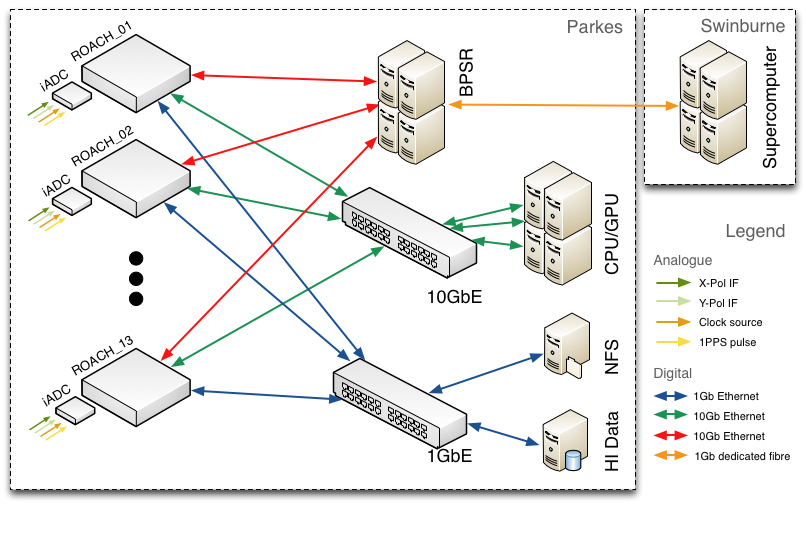
\includegraphics{HIPSR_arch.png}
\caption{\emph{Network architecture for HIPSR.}}\end{figure}

\begin{notice}{note}{Note:}
The GPU servers are mainly used for pulsar work. All of the signal processing for HISPEC
(HI spectrometer) is currently done on the CASPER ROACH boards. Future (lower bandwidth)
modes of observation will likely use the GPU servers too.
\end{notice}


\section{Software}
\label{user_guide:software}
If you \emph{really} want to know
what's going on, the module listing and API can be found here: {\hyperref[software:software-chapter]{\emph{Software}}}.
A quick run-through is shown below.


\subsection{hipsr-server.py}
\label{user_guide:hipsr-server-py}
For HISPEC, all of the signal processing is done on the ROACH boards. The ROACH boards are
controlled by a script, \emph{hipsr-server.py}, which collects data from the ROACH boards and
metadata (e.g. pointing info) from the telescope control system (TCS). The server script then
writes the data to HDF5 files. Note that \emph{hipsr-server.py} does not control telescope pointing,
it only collects and collates data/metadata.


\subsection{hipsr-gui.py}
\label{user_guide:hipsr-gui-py}
Data from HISPEC can be monitored using the \emph{hipsr-gui.py} script. This script gives shows the
bandpass from all 13 beams, and has a beam scope, waterfall plotter and total power monitor.
\begin{figure}[htbp]
\centering
\capstart

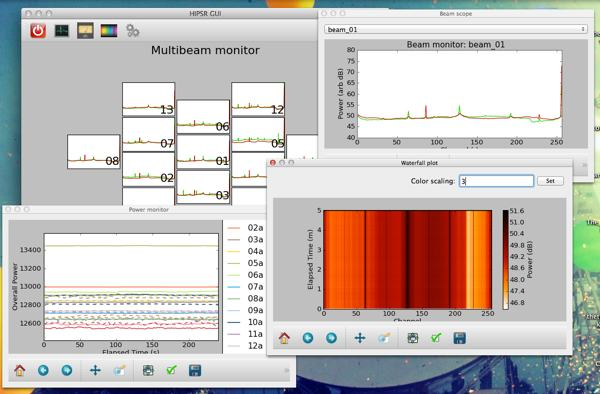
\includegraphics{hipsr-gui.jpg}
\caption{\emph{Screenshot of hipsr-gui running on Mac OSX.}}\end{figure}


\subsection{hipsr-writer.py}
\label{user_guide:hipsr-writer-py}
The \emph{hipsr-writer.py} script converts files from HDF5 to SD-FITS. At the end of your observations, you'll want to run this as most data reduction packages don't support HDF5 yet.

\begin{notice}{note}{Note:}
All firmware and software for HIPSR is stored on github: \href{https://github.com/telegraphic/hipsr}{https://github.com/telegraphic/hipsr}.
It is of course, already installed wherever it needs to be.
\end{notice}


\section{How everything fits together}
\label{user_guide:how-everything-fits-together}\begin{figure}[htbp]
\centering
\capstart

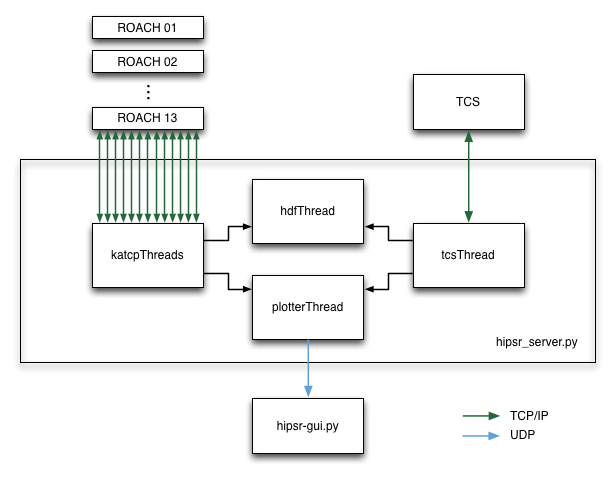
\includegraphics{hipsr-server.png}
\caption{\emph{What's really going on.}}\end{figure}

The hipsr-server collects, collates and writes data to HDF files. To do this, several threads must be run in parallel. Firstly, a connection to each ROACH board is made using \href{https://casper.berkeley.edu/wiki/KATCP}{KATCP}, a communication
protocol which runs over TCP/IP. Each connection runs in a separate thread. In addition to this, a
TCP/IP server is set up to communicate with TCS, which sends ASCII command : value pairs with info
about telescope setup, observation config and pointing detiails.

Having multiple threads all attempting to write the same HDF file isn't good. So, there's a dedicated
HDF thread which has a data input queue, into which the KATCP and TCS threads append data. Finally,
so we can see what's going on, TCS and KATCP threads send a subset of data over a UDP connection to
the {\hyperref[user_guide:hipsr-gui-py]{hipsr-gui.py}} script, which is generally run on a different computer. This UDP connection sends
python dictionaries converted into JSON.


\section{Observing with HIPSR}
\label{user_guide:observing-with-hipsr}

\subsection{Starting observations}
\label{user_guide:starting-observations}
There are three things that must be started to observe with HIPSR:
\begin{enumerate}
\item {} 
The telescope control system, TCS

\item {} 
The hipsr-server script which runs on hipsr-srv0

\item {} 
The hipsr-gui plotter which runs on {[}?{]}

\end{enumerate}

To start TCS, get onto one of the Sun machines and type:

\begin{Verbatim}[commandchars=\\\{\}]
\textgreater{} tcs
\end{Verbatim}

Until someone copy and paste's how to use TCS here, you'll have to consult the \href{http://www.parkes.atnf.csiro.au/observing/documentation/user\_guide/}{telescope user guide}.

\emph{Before} you press ``go'' on TCS, you first need to start the hipsr-server script. To do so,
you need to SSH into hipsr-srv0:

\begin{Verbatim}[commandchars=\\\{\}]
\textgreater{} ssh [user]@hipsr-srv0(.atnf.csiro.au)
\end{Verbatim}

Once you've connected, change into directory /data/hipsr/hipsr-server/:

\begin{Verbatim}[commandchars=\\\{\}]
\textgreater{} cd /data/hipsr/hipsr-server/
\end{Verbatim}

Finally, start the server with the command:

\begin{Verbatim}[commandchars=\\\{\}]
\textgreater{} ./hipsr\_server.py
\end{Verbatim}

You can optionally pass the argument -p PXXX, where PXXX is your project ID, e.g.:

\begin{Verbatim}[commandchars=\\\{\}]
\textgreater{} ./hipsr\_server.py -p P641
\end{Verbatim}

This might save you a few seconds.


\subsection{Stopping observations}
\label{user_guide:stopping-observations}
To stop the server, press ctrl + C. The server will close all open files before exiting.


\subsection{Getting your data}
\label{user_guide:getting-your-data}
HIPSR data is stored on hipsr-srv0 in /data/hipsr/.


\section{When things go wrong}
\label{user_guide:when-things-go-wrong}
Here's a few notes on problems you might run into with HIPSR. For anything to do with the
telescope, consult the \href{http://www.parkes.atnf.csiro.au/observing/documentation/user\_guide/}{telescope user guide}.


\subsection{Socket errors}
\label{user_guide:socket-errors}
TCS seems to give a random socket error 9: bad file name the first time
it connects to the HIPSR server (hipsr-srv0). This doesn't seem to matter.

Sometimes the TCS socket (59012) is held open, and neither TCS or HIPSR will negotiate
a new TCP/IP connection. If this happens, you can check the port status by typing:

\begin{Verbatim}[commandchars=\\\{\}]
\textgreater{} netstat \textbar{} grep 59012
\end{Verbatim}

You can check whether there's another instance of hipsr\_server by typing:

\begin{Verbatim}[commandchars=\\\{\}]
\textgreater{} ps aux \textbar{} grep hipsr\_server
\end{Verbatim}

\begin{notice}{caution}{Caution:}
If there's a rogue instance of hipsr-sever.py running, you may have to kill it.
This can be done with the command:

\begin{Verbatim}[commandchars=\\\{\}]
\textgreater{} kill [PID]
\end{Verbatim}

However, take care when doing this that you kill the right thing.
\end{notice}


\chapter{Hardware}
\label{hardware:hardware-chapter}\label{hardware:hardware}\label{hardware:telescope-user-guide}\label{hardware::doc}
This page details the hardware in use in the HIPSR system. HIPSR consists of digitizer
cards; FPGA digital processing boards for ``low-level'' DSP; a 10GbE switch for data
interconnect; and, a CPU/GPU cluster for ``high-level'' DSP and data storage.


\section{HIPSR Packetized Architecture}
\label{hardware:hipsr-packetized-architecture}\begin{figure}[htbp]
\centering
\capstart

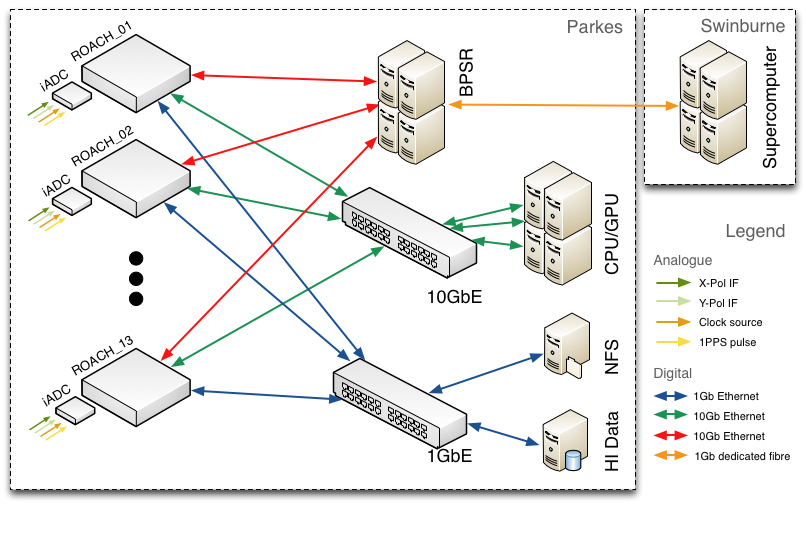
\includegraphics{HIPSR_arch.png}
\caption{\emph{Network architecture for HIPSR.}}\end{figure}

The HIPSR system may be described as a multi-node DSP {\color{red}\bfseries{}{}`}frontend' connected to a multi-node DSP {\color{red}\bfseries{}{}`}backend' by a 10Gb Ethernet (10GbE) switch. In the HIPSR system detailed here, DSP tasks are divided between FPGAs and GPGPUs as appropriate. The FPGA based DSP frontend conducts signal processing tasks such as signal filtering and channelization; the GPGPU based DSP backend performs higher-level, moderate- to low- bandwidth DSP such as running pulsar processing pipelines. A diagram of the system archiecture is shown below.

The inclusion of a switch greatly increases the flexibility of the system as data can be dynamically routed between nodes. It does, however, require all data to be packetized along with metadata that describes packet's data payload. Nevertheless, using a switched 10GbE based packetized architecture instead of defining and commissioning a bespoke backplane has drastically decreased development time: all interconnect is off-the-shelf, industry standard, commodity hardware.


\section{CASPER ROACH boards}
\label{hardware:casper-roach-boards}\begin{figure}[htbp]
\centering
\capstart

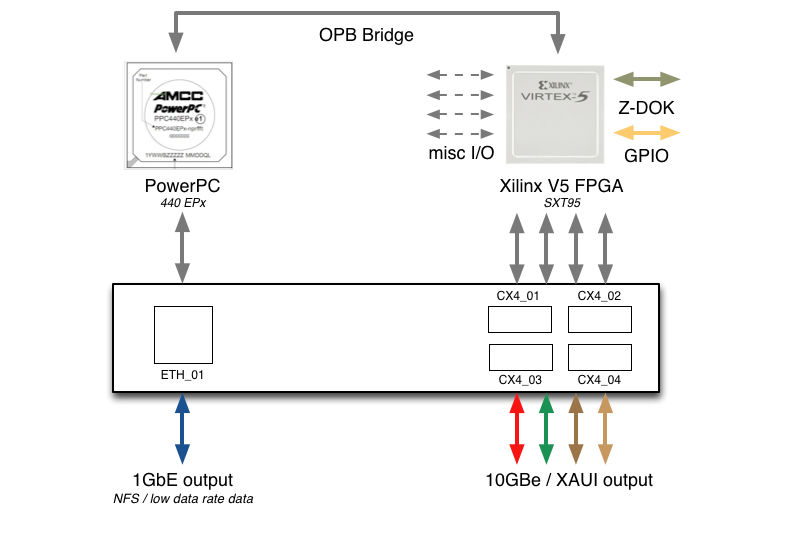
\includegraphics{ROACH_IO.png}
\caption{\emph{Roach Input/Output}}\end{figure}

ROACH (Reconfigurable Open Architecture Computing Hardware) is a standalone
FPGA processing board, developed by the Collaboration for Astronomy Signal Processing
and Electronics Research.

The centrepiece of ROACH is a Xilinx Virtex 5 FPGA (SX95T).
A separate PowerPC runs Linux and is used to control the board (program the FPGA
and allow interfacing between the FPGA ``software registers/BRAMs/FIFOs'' and external
devices using Ethernet).

Two quad data rate (QDR) SRAMs provide high-speed, medium-capacity memory
(specifically for doing corner-turns), and one DDR2 DIMM provides slower-speed,
high-capacity buffer memory for the FPGA. The PowerPC has an independent DDR2 DIMM
in order to boot Linux/BORPH.

The two Z-DOK connectors allow ADC, DAC and other interface cards to be attached to the
FPGA, in the same manner as the IBOB allowed (with backwards compatibility for the ADC
boards used with the IBOB).

Four CX4 connectors provide a total of 40Gbits/sec bandwidth for connecting ROACH boards
together, or connecting them to other XAUI/10GbE-capable devices (such as
computers with 10GbE NICs and 10GbE switches).

For more detailed descriptions, see:
\begin{itemize}
\item {} 
\href{https://casper.berkeley.edu/wiki/Main\_Page}{https://casper.berkeley.edu/wiki/Main\_Page}

\item {} 
\href{https://casper.berkeley.edu/wiki/ROACH}{https://casper.berkeley.edu/wiki/ROACH}

\item {} 
\href{https://casper.berkeley.edu/wiki/ROACH\_Architecture}{https://casper.berkeley.edu/wiki/ROACH\_Architecture}

\end{itemize}


\section{iADC digitizer cards}
\label{hardware:iadc-digitizer-cards}
Each HIPSR ROACH board is populated with an iADC digitizer card. These cards are
based on the Atmel/e2V AT84AD001B 8-bit Dual 1Gsps ADC:
\begin{itemize}
\item {} 
\href{http://www.e2v.com/assets/media/files/documents/broadband-data-converters/doc0817I.pdf}{http://www.e2v.com/assets/media/files/documents/broadband-data-converters/doc0817I.pdf}

\end{itemize}

More information about the card is available at:
\begin{itemize}
\item {} 
\href{https://casper.berkeley.edu/wiki/ADC2x1000-8}{https://casper.berkeley.edu/wiki/ADC2x1000-8}

\end{itemize}


\section{Cisco switch}
\label{hardware:cisco-switch}
The DSP frontend and backend nodes are connected via a 10Gb Ethernet switch. This Cisco 4900M switch is configured with 24 CX4-type ports, 13 of which are connected to the DSP frontend ROACH boards, and 8 of which are connected to the server nodes. The switch allows bi-directional data flow between nodes. The 10GbE switch also has a dedicated 1GbE fibre link to the \href{http://astronomy.swin.edu.au/supercomputing/green2/}{Green II supercomputer}

at Swinburne University in Melbourne.

All nodes are also connected by 1GbE, through a Cisco 3750 switch. For low bandwidth applications where all of the necessary DSP can be conducted on the FPGA, all data may be read off the 1GbE ports of the ROACH boards.

\begin{tabulary}{\linewidth}{|L|L|}
\hline
\textbf{
Item
} & \textbf{
Description
}\\\hline

WS-C4900M
 & 
CISCO Base system with 8 X2 ports and 2 half slots
\\\hline

S49MIPBK9-15002SG
 & 
CISCO Cisco CAT4900M IOS IP BASE SSH
\\\hline

PWR-C49M-1000AC
 & 
CISCO 4900M AC power supply, 1000 watts
\\\hline

PWR-C49M-1000AC/2
 & 
CISCO Redundant AC PS for 4900M
\\\hline

CAB-AS3112-C15-AU
 & 
CISCO AS-3112 to IEC-C15 8ft Aus
\\\hline

MEM-C4K-FLD128M
 & 
CISCO Catalyst 4900M Compact Flash, 128MB Option
\\\hline

4900M-X2-CVR
 & 
CISCO X2 cover on 4900M
\\\hline

WS-X4908-10GE=
 & 
CISCO 8 port 2:1 10GbE (X2) line card for 4900M series
(this is the expansion module - there are two slots
in each chassis)
\\\hline
\end{tabulary}



\section{HIPSR Servers}
\label{hardware:hipsr-servers}

\subsection{Server nodes}
\label{hardware:server-nodes}
The GPGPU server nodes are bespoke systems, built to specification by Silicon Graphics Pty. Ltd. Each of the 8 server nodes are comprised of:
\begin{itemize}
\item {} 
dual 2.66 GHz Intel Xeon six-core CPUs,

\item {} 
48 GB DDR3 memory, and

\item {} 
dual Nvidia Tesla C2070 GPGPUs.

\end{itemize}

While it is intended that a majority of DSP will be conducted on the GPGPUs, the Intel Xeon CPUs may also be used, if required.

As each server has a single CX4-type 10GbE network interface card (NIC), the input data rate for each server is limited to 10 Gb/s. Given that there are 26 IFs which must be processed by 8 server nodes, the DSP frontend must decrease the data rate of
\begin{quote}

\textbf{2 x 400MHz x 8bit = 6.4 Gb/s}
\end{quote}

from each IF from 6.4Gb/s to about 3.0Gb/s.


\subsection{hipsr-srv0}
\label{hardware:hipsr-srv0}
In addition to the GPGPU server nodes, there is a server which provides monitor and control for the DSP frontend, and provides data storage. This server has:
\begin{itemize}
\item {} 
a 2.4 GHz Intel Xeon four-core CPU,

\item {} 
24 GB DDR3 memory,

\item {} 
5TB RAID HDD

\end{itemize}

As it is not used for DSP, it does not have a GPGPU. This server runs a DHCP daemon and provides a network file system (NFS) to the ROACH boards.


\section{Cabling}
\label{hardware:cabling}
In March 2012, the HIPSR hardware was installed into RFI shielded racks R and S, located on the second floor of the Parkes 64m telescope building (this room lies underneath the telescope dish).
* A set of BNC cables were laid under the floor from the existing multibeam IF distribution panel to BNC feedthroughs installed on the racks.
* Another set of cables connect the BNC feedthrough to the SMA input of the iADC cards.
* A third set of cables connects the 1PPS input of the iADC to a PPS distribution unit, and a clock signal is distributed to each board by a fourth set of SMA cables.

Each server node and ROACH board is connected to a 1GbE switch by an Ethernet cable (CAT-5E STP). Similarly, each server node and ROACH is connected to a 10GbE switch via CX4 type cables.


\chapter{Software}
\label{software:module-hipsr_server}\label{software:software}\label{software::doc}\label{software:software-chapter}\index{hipsr\_server (module)}

\section{hipsr\_server.py}
\label{software:hipsr-server-py}
HIPSR wideband spectrometer server script. This script reprograms and reconfigures the roach
boards, creates a data file, and then begins collecting data from TCS and the roach boards.

A seperate thread is created for each roach board, so that reading and writing data can be done
in parallel. In addition, there is a thread which acts as a server that listend for TCS messages.
To write to the HDF data file, these threads append an I/O requests to a FIFO (Queue.Queue) which
is constantly checked by yet another thread.

Created by Danny Price on 2011-10-05.
Copyright (c) 2012 The HIPSR collaboration. All rights reserved.
\index{DataFetcher (class in hipsr\_server)}

\begin{fulllineitems}
\phantomsection\label{software:hipsr_server.DataFetcher}\pysiglinewithargsret{\strong{class }\code{hipsr\_server.}\bfcode{DataFetcher}}{\emph{queue}}{}
Thread worker function for retrieving data from roach boards
\paragraph{Methods}
\index{run() (hipsr\_server.DataFetcher method)}

\begin{fulllineitems}
\phantomsection\label{software:hipsr_server.DataFetcher.run}\pysiglinewithargsret{\bfcode{run}}{}{}
Thread run method. Fetch data from roach

\end{fulllineitems}


\end{fulllineitems}

\index{Logger (class in hipsr\_server)}

\begin{fulllineitems}
\phantomsection\label{software:hipsr_server.Logger}\pysiglinewithargsret{\strong{class }\code{hipsr\_server.}\bfcode{Logger}}{\emph{filename}, \emph{filepath}}{}
Logger which records the output of stdin to file
\paragraph{Methods}

\end{fulllineitems}

\index{createNewFile() (in module hipsr\_server)}

\begin{fulllineitems}
\phantomsection\label{software:hipsr_server.createNewFile}\pysiglinewithargsret{\code{hipsr\_server.}\bfcode{createNewFile}}{}{}
Closes current file and creates a new one

\end{fulllineitems}

\index{getSpectraThreaded() (in module hipsr\_server)}

\begin{fulllineitems}
\phantomsection\label{software:hipsr_server.getSpectraThreaded}\pysiglinewithargsret{\code{hipsr\_server.}\bfcode{getSpectraThreaded}}{\emph{fpgalist}, \emph{queue}}{}
Retrieves spectral data from multiple roach boards

Spawns multiple threads, with each thread retrieving from a single board.
A queue is used to block until all threads have completed.

\end{fulllineitems}

\index{hdfWriter() (in module hipsr\_server)}

\begin{fulllineitems}
\phantomsection\label{software:hipsr_server.hdfWriter}\pysiglinewithargsret{\code{hipsr\_server.}\bfcode{hdfWriter}}{}{}
Worker thread that writes to HDF files

\end{fulllineitems}

\index{tcsServer() (in module hipsr\_server)}

\begin{fulllineitems}
\phantomsection\label{software:hipsr_server.tcsServer}\pysiglinewithargsret{\code{hipsr\_server.}\bfcode{tcsServer}}{}{}
A TCP server which listens for TCS commands and parses them

\end{fulllineitems}

\index{toJson() (in module hipsr\_server)}

\begin{fulllineitems}
\phantomsection\label{software:hipsr_server.toJson}\pysiglinewithargsret{\code{hipsr\_server.}\bfcode{toJson}}{\emph{npDict}}{}
Converts a dictionary of numpy arrays into a dictionary of lists.

\end{fulllineitems}

\phantomsection\label{software:module-hipsr_gui}\index{hipsr\_gui (module)}

\section{hipsr\_gui.py}
\label{software:hipsr-gui-py}
This script starts a Qt4 + matplotlib based graphical user interface for monitoring HIPSR's data output.


\subsection{Requirements}
\label{software:requirements}
PySide (or PyQt), for Qt4 bindings
numpy, matplotlib.


\subsection{TODO:}
\label{software:todo}\begin{itemize}
\item {} 
Zoom in on selected area

\item {} 
Tabbed versions

\item {} 
Pause \& explore plot

\item {} 
save image

\item {} 
show which beam is which

\end{itemize}
\index{HipsrGui (class in hipsr\_gui)}

\begin{fulllineitems}
\phantomsection\label{software:hipsr_gui.HipsrGui}\pysigline{\strong{class }\code{hipsr\_gui.}\bfcode{HipsrGui}}
HIPSR GUI class

A Qt4 Widget that uses matplotlib to display data from UDP packets.
\paragraph{Methods}
\index{bufferUDPData() (hipsr\_gui.HipsrGui method)}

\begin{fulllineitems}
\phantomsection\label{software:hipsr_gui.HipsrGui.bufferUDPData}\pysiglinewithargsret{\bfcode{bufferUDPData}}{}{}
A circular buffer for incoming UDP packets

\end{fulllineitems}

\index{createMultiBeamPlot() (hipsr\_gui.HipsrGui method)}

\begin{fulllineitems}
\phantomsection\label{software:hipsr_gui.HipsrGui.createMultiBeamPlot}\pysiglinewithargsret{\bfcode{createMultiBeamPlot}}{\emph{numchans=256}}{}
Creates 13 subplots in a hexagonal array representing the multibeam feeds

\end{fulllineitems}

\index{createOverallPowerPlot() (hipsr\_gui.HipsrGui method)}

\begin{fulllineitems}
\phantomsection\label{software:hipsr_gui.HipsrGui.createOverallPowerPlot}\pysiglinewithargsret{\bfcode{createOverallPowerPlot}}{\emph{numchans=120}, \emph{beamid='beam\_01'}}{}
Creates an overall power vs time plot.

\end{fulllineitems}

\index{createSingleBeamPlot() (hipsr\_gui.HipsrGui method)}

\begin{fulllineitems}
\phantomsection\label{software:hipsr_gui.HipsrGui.createSingleBeamPlot}\pysiglinewithargsret{\bfcode{createSingleBeamPlot}}{\emph{numchans=256}, \emph{beamid='beam\_01'}}{}
Creates a single pylab plot for HIPSR data.

\end{fulllineitems}

\index{createWaterfallPlot() (hipsr\_gui.HipsrGui method)}

\begin{fulllineitems}
\phantomsection\label{software:hipsr_gui.HipsrGui.createWaterfallPlot}\pysiglinewithargsret{\bfcode{createWaterfallPlot}}{}{}
Creates a single imshow plot for HIPSR data.

\end{fulllineitems}

\index{initUI() (hipsr\_gui.HipsrGui method)}

\begin{fulllineitems}
\phantomsection\label{software:hipsr_gui.HipsrGui.initUI}\pysiglinewithargsret{\bfcode{initUI}}{\emph{width=1200}, \emph{height=750}}{}
Initialize the User Interface
\begin{quote}\begin{description}
\item[{Parameters }] \leavevmode
\textbf{width: int} :
\begin{quote}

width of the UI, in pixels. Defaults to 1024px
\end{quote}

\textbf{height: int} :
\begin{quote}

height of the UI, in pixels. Defaults to 768px
\end{quote}

\end{description}\end{quote}

\end{fulllineitems}

\index{onBeamSelect() (hipsr\_gui.HipsrGui method)}

\begin{fulllineitems}
\phantomsection\label{software:hipsr_gui.HipsrGui.onBeamSelect}\pysiglinewithargsret{\bfcode{onBeamSelect}}{\emph{beam}}{}
Beam selection combo box actions

\end{fulllineitems}

\index{updateAllPlots() (hipsr\_gui.HipsrGui method)}

\begin{fulllineitems}
\phantomsection\label{software:hipsr_gui.HipsrGui.updateAllPlots}\pysiglinewithargsret{\bfcode{updateAllPlots}}{}{}
Redraw all graphs in GUI

\end{fulllineitems}

\index{updateOverallPowerPlot() (hipsr\_gui.HipsrGui method)}

\begin{fulllineitems}
\phantomsection\label{software:hipsr_gui.HipsrGui.updateOverallPowerPlot}\pysiglinewithargsret{\bfcode{updateOverallPowerPlot}}{\emph{key}, \emph{xx}, \emph{yy}}{}
Update power monitor plot.

\end{fulllineitems}

\index{updateWaterfallPlot() (hipsr\_gui.HipsrGui method)}

\begin{fulllineitems}
\phantomsection\label{software:hipsr_gui.HipsrGui.updateWaterfallPlot}\pysiglinewithargsret{\bfcode{updateWaterfallPlot}}{\emph{new\_data}}{}
Updates waterfall plot with new values

\end{fulllineitems}

\index{updateWaterfallThreshold() (hipsr\_gui.HipsrGui method)}

\begin{fulllineitems}
\phantomsection\label{software:hipsr_gui.HipsrGui.updateWaterfallThreshold}\pysiglinewithargsret{\bfcode{updateWaterfallThreshold}}{}{}
Change the threshold value for the waterfall plot

\end{fulllineitems}


\end{fulllineitems}



\chapter{Gateware}
\label{gateware::doc}\label{gateware:gateware}

\section{Overview}
\label{gateware:overview}
The MSSGE toolflow (short for Matlab/Simulink/System Generator/EDK) is the platform
for FPGA-based CASPER development, which stitches together several design and implementation
environments.

It is better known as the bee\_xps toolflow, which was developed at the Berkeley Wireless
Research Center (BWRC) as a high-level design tool for the BEE and BEE2 platforms. We have
extended it to work with all other CASPER boards as well. It provides a graphical
Matlab/Simulink design environment using the Xilinx System Generator Toolbox,
and abstracts the Xilinx implementation details behind a one-click compile interface.

For installation instructions, see the MSSGE Toolflow page:
\begin{itemize}
\item {} 
\href{https://casper.berkeley.edu/wiki/MSSGE\_Toolflow}{https://casper.berkeley.edu/wiki/MSSGE\_Toolflow}

\end{itemize}


\section{Spectral line modes}
\label{gateware:spectral-line-modes}

\subsection{HIPSR Wideband Spectrometer}
\label{gateware:hipsr-wideband-spectrometer}
\textbf{Current gateware: hipsr\_16\_2011\_Oct\_01\_0824.bof}

This is a 400MHz bandwidth, 8192 channel polyphase filterbank. The filterbank
is 4-taps, with hamming window coefficients.
\begin{figure}[htbp]
\centering
\capstart

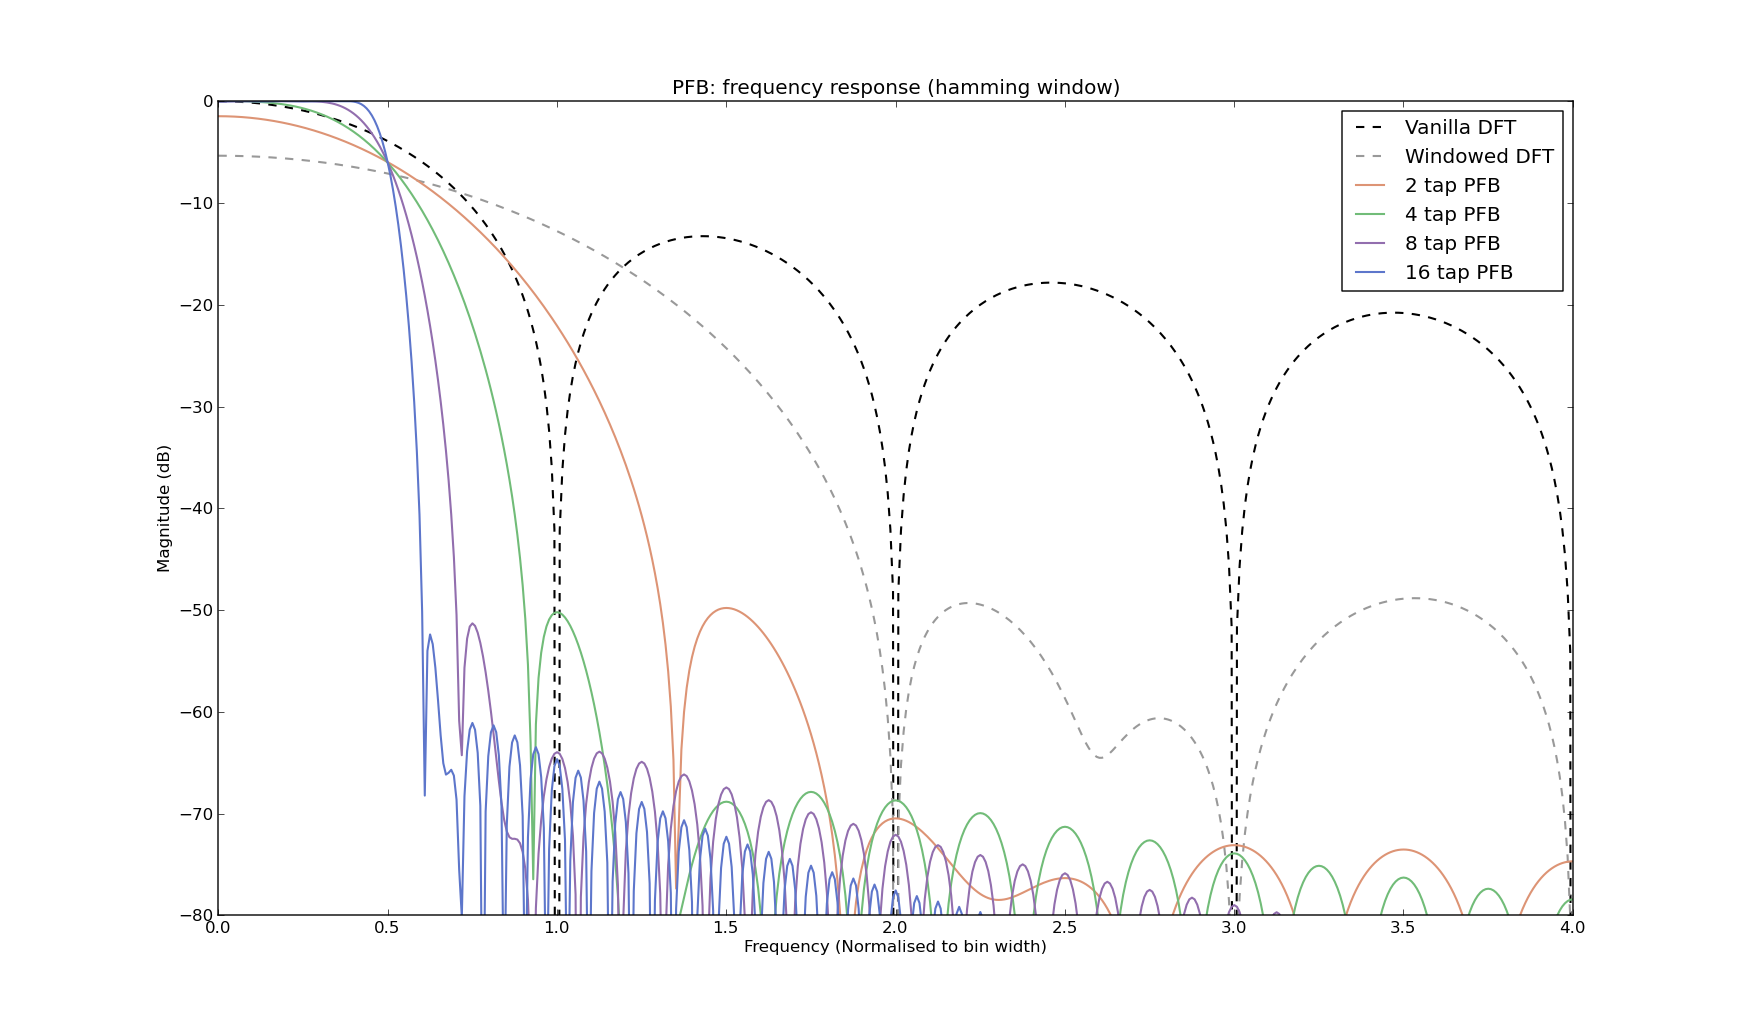
\includegraphics{PFB_response.png}
\caption{\emph{Filterbank response for different numbers of taps. We are using 4-taps in
this 8192 channel design.}}\end{figure}

The registers that can be used to control the board logic are listed below.

\begin{tabulary}{\linewidth}{|L|L|}
\hline
\textbf{
Register
} & \textbf{
Description
}\\\hline

quant\_gain
 & 
Gain used in quantization, accepts an eight bit
number which sets the shift before quantisation.
Values under 00001111 shift the data to the left;
values over  00001111 shift the data to the right.
\\\hline

mux\_sel
 & 
Digital noise source or the ADC? A value of 1 selects
the digital noise source, and 0 selects the ADC input.
\\\hline

fft\_shift
 & 
FFT shift, selects which stages of the FFT the bits are
shifter to the left. Accepts 12 bits, one bit for each
stage in the FFT. For example, 111111111111 shifts every
stage, and 010101010101 shifts every second stage.
\\\hline

acc\_len
 & 
Number of accumulations, in clock cycles. As the FPGA
is clocked at 200MHz, and there are 8192 channels, a
value of 24414 corresponds to 1 second. The maximum
value is 2\textasciicircum{}18 accumulations, which gives about 10s,
although care must be taken to ensure there is no overflow.
\\\hline
\end{tabulary}


\textbf{Resource utilization summary}

The design uses a fair proportion of slices and BRAMs, but there is a fair
amount of DSP48E logic left.

\begin{tabulary}{\linewidth}{|L|L|L|}
\hline
\textbf{
Logic distribution and feature utilization
} & \textbf{} & \textbf{}\\\hline

Number of occupied Slices:
 & 
10,305 out of  14,720
 & 
70\%
\\\hline

Number of LUT Flip Flop pairs used:
 & 
36,261
 & \\\hline

Number with an unused Flip Flop:
 & 
2,830 out of  36,261
 & 
7\%
\\\hline

Number with an unused LUT:
 & 
9,846 out of  36,261
 & 
27\%
\\\hline

Number of fully used LUT-FF pairs:
 & 
23,585 out of  36,261
 & 
65\%
\\\hline

Number of unique control sets:
 & 
167
 & \\\hline

Number of slice register sites lost
 &  & \\\hline

to control set restrictions:
 & 
229 out of  58,880
 & 
1\%
\\\hline

Number of BlockRAM/FIFO:
 & 
191 out of     244
 & 
78\%
\\\hline

Number using BlockRAM only:
 & 
191
 & \\\hline

Total primitives used:
 &  & \\\hline

Number of 36k BlockRAM used:
 & 
185
 & \\\hline

Number of 18k BlockRAM used:
 & 
12
 & \\\hline

Total Memory used (KB):
 & 
6,876 out of   8,784
 & 
78\%
\\\hline

Number of DSP48Es:
 & 
222 out of     640
 & 
34\%
\\\hline
\end{tabulary}



\section{Pulsar modes}
\label{gateware:pulsar-modes}
The CASPSR firmware is based on the Packetized Astronomy Signal Processor
firmware designed by Terry Filiba. The BPSR firmware is based on the Parspec
firmware designed by Peter Macmahon and ported to ROACH by Danny Price.


\subsection{ADC to Ten Gigabit Ethernet}
\label{gateware:adc-to-ten-gigabit-ethernet}
\textbf{Current gateware: adc\_to\_10gbe\_2011\_Oct\_18\_1156.bof}

CASPSR uses a stripped out PASP. It has a more accurate reset, and just turns the ADC input
into 10GE packets.
\begin{itemize}
\item {} 
\href{https://casper.berkeley.edu/wiki/Packetized\_Astronomy\_Signal\_Processor}{https://casper.berkeley.edu/wiki/Packetized\_Astronomy\_Signal\_Processor}

\end{itemize}

\begin{tabulary}{\linewidth}{|L|L|}
\hline
\textbf{
Register
} & \textbf{
Description
}\\\hline

todo
 & 
todo.
\\\hline
\end{tabulary}


\textbf{Resource utilization summary}

This design fitted onto an iBOB, so unsuprisingly isn't pushing the ROACH in any
way.

\begin{tabulary}{\linewidth}{|L|L|L|}
\hline
\textbf{
Logic distribution and feature utilization
} & \textbf{} & \textbf{}\\\hline

Number of occupied Slices:
 & 
6,258 out of  14,720
 & 
42\%
\\\hline

Number of LUT Flip Flop pairs used:
 & 
16,637
 & \\\hline

Number with an unused Flip Flop:
 & 
6,747 out of  16,637
 & 
40\%
\\\hline

Number with an unused LUT:
 & 
3,378 out of  16,637
 & 
20\%
\\\hline

Number of fully used LUT-FF pairs:
 & 
6,512 out of  16,637
 & 
39\%
\\\hline

Number of unique control sets:
 & 
459
 & \\\hline

Number of slice register sites lost
 &  & \\\hline

to control set restrictions:
 & 
1,041 out of  58,880
 & 
1\%
\\\hline

Number of BlockRAM/FIFO:
 & 
21 out of     244
 & 
8\%
\\\hline

Number using BlockRAM only:
 & 
21
 & \\\hline

Total primitives used:
 &  & \\\hline

Number of 36k BlockRAM used:
 & 
12
 & \\\hline

Number of 18k BlockRAM used:
 & 
16
 & \\\hline

Total Memory used (KB):
 & 
720 out of   8,784
 & 
8\%
\\\hline
\end{tabulary}



\subsection{Parkes Spectrometer (Parspec)}
\label{gateware:parkes-spectrometer-parspec}
\textbf{Current gateware: parspec\_01\_2011\_Oct\_12\_1520.bof}

Parspec is a 400MHz bandwidth, 1024 channel, 2-tap polyphase filterbank based
spectrometer.
\begin{itemize}
\item {} 
\href{https://casper.berkeley.edu/wiki/Parspec}{https://casper.berkeley.edu/wiki/Parspec}

\end{itemize}

\begin{tabulary}{\linewidth}{|L|L|}
\hline
\textbf{
Register
} & \textbf{
Description
}\\\hline

todo
 & 
todo.
\\\hline
\end{tabulary}


\textbf{Resource utilization summary}

Parspec was designed and spec'd to fit onto an iBOB; now it's been ported to
ROACH it feels positively roomy.

\begin{tabulary}{\linewidth}{|L|L|L|}
\hline
\textbf{
Logic distribution and feature utilization
} & \textbf{} & \textbf{}\\\hline

Number of occupied Slices:
 & 
6,171 out of  14,720
 & 
41\%
\\\hline

Number of LUT Flip Flop pairs used:
 & 
20,028
 & \\\hline

Number with an unused Flip Flop:
 & 
3,139 out of  20,028
 & 
15\%
\\\hline

Number with an unused LUT:
 & 
5,881 out of  20,028
 & 
29\%
\\\hline

Number of fully used LUT-FF pairs:
 & 
11,008 out of  20,028
 & 
54\%
\\\hline

Number of unique control sets:
 & 
349
 & \\\hline

Number of slice register sites lost
 &  & \\\hline

to control set restrictions:
 & 
728 out of  58,880
 & 
1\%
\\\hline

Number of BlockRAM/FIFO:
 & 
85 out of     244
 & 
34\%
\\\hline

Number using BlockRAM only:
 & 
85
 & \\\hline

Total primitives used:
 &  & \\\hline

Number of 36k BlockRAM used:
 & 
10
 & \\\hline

Number of 18k BlockRAM used:
 & 
119
 & \\\hline

Total Memory used (KB):
 & 
2,502 out of   8,784
 & 
28\%
\\\hline

Number of DSP48Es:
 & 
164 out of     640
 & 
25\%
\\\hline
\end{tabulary}



\chapter{Roach Setup/Config}
\label{ip_allocation:roach-setup-config}\label{ip_allocation::doc}

\section{IF mappings}
\label{ip_allocation:if-mappings}
\begin{tabulary}{\linewidth}{|L|L|L|L|L|L|L|L|}
\hline
\textbf{
I
} & \textbf{
Q
} & \textbf{
beam ID
} & \textbf{
hostname
} & \textbf{
nickname
} & \textbf{
Rack
} & \textbf{
iADC
} & \textbf{
ADC notes
}\\\hline

1
 & 
2
 & 
beam\_01
 & 
roach040149
 & 
Drake
 & 
R
 & 
iADC v1.1a
 & 
oxford loan
\\\hline

3
 & 
4
 & 
beam\_02
 & 
roach040150
 & 
Hendrix
 & 
R
 & 
iADC v1.1a
 & 
oxford loan
\\\hline

5
 & 
6
 & 
beam\_03
 & 
roach040151
 & 
Keenan
 & 
R
 & 
iADC v1.1a
 & 
oxford loan
\\\hline

7
 & 
8
 & 
beam\_04
 & 
roach040152
 & 
Mackaye
 & 
R
 & 
iADC v1.1a
 & 
oxford loan
\\\hline

9
 & 
10
 & 
beam\_05
 & 
roach040154
 & 
Reznor
 & 
R
 & 
iADC v1.1a
 & 
oxford loan
\\\hline

11
 & 
12
 & 
beam\_06
 & 
roach040155
 & 
Barrett
 & 
S
 & 
iADC v1.1a
 & 
BPSR spare
\\\hline

13
 & 
14
 & 
beam\_07
 & 
roach040148
 & 
Curtis
 & 
S
 & 
iADC v 1.1b
 & 
HIPSR
\\\hline

15
 & 
16
 & 
beam\_08
 & 
roach040140
 & 
Albarn
 & 
S
 & 
iADC v 1.1b
 & 
HIPSR
\\\hline

17
 & 
18
 & 
beam\_09
 & 
roach040158
 & 
Willis
 & 
S
 & 
iADC v1.1a
 & 
oxford loan
\\\hline

19
 & 
20
 & 
beam\_10
 & 
roach040157
 & 
Waits
 & 
S
 & 
iADC v1.1a
 & 
oxford loan
\\\hline

21
 & 
22
 & 
beam\_11
 & 
roach040156
 & 
Yorke
 & 
S
 & 
iADC v 1.1b
 & 
HIPSR
\\\hline

23
 & 
24
 & 
beam\_12
 & 
roach040146
 & 
Cobain
 & 
S
 & 
iADC v1.1a
 & 
oxford loan
\\\hline

25
 & 
26
 & 
beam\_13
 & 
roach040147
 & 
Cohen
 & 
S
 & 
iADC v1.1a
 & 
oxford loan
\\\hline
\end{tabulary}


TODO: Check and update


\section{IP Address Allocation}
\label{ip_allocation:ip-address-allocation}
\begin{tabulary}{\linewidth}{|L|L|L|L|L|}
\hline
\textbf{
hostname
} & \textbf{
nickname
} & \textbf{
Eth0 MAC
} & \textbf{
Eth0 IP
} & \textbf{
Xport IP
}\\\hline

roach040149
 & 
Drake
 & 
02:00:00:04:01:49
 & 
192.168.1.149
 & 
192.168.1.49
\\\hline

roach040150
 & 
Hendrix
 & 
02:00:00:04:01:50
 & 
192.168.1.150
 & 
192.168.1.50
\\\hline

roach040151
 & 
Keenan
 & 
02:00:00:04:01:51
 & 
192.168.1.151
 & 
192.168.1.51
\\\hline

roach040152
 & 
Mackaye
 & 
02:00:00:04:01:52
 & 
192.168.1.152
 & 
192.168.1.52
\\\hline

roach040154
 & 
Reznor
 & 
02:00:00:04:01:54
 & 
192.168.1.154
 & 
192.168.1.54
\\\hline

roach040155
 & 
Barrett
 & 
02:00:00:04:01:55
 & 
192.168.1.155
 & 
192.168.1.55
\\\hline

roach040148
 & 
Curtis
 & 
02:00:00:04:01:48
 & 
192.168.1.148
 & 
192.168.1.48
\\\hline

roach040140
 & 
Albarn
 & 
02:00:00:04:01:40
 & 
192.168.1.140
 & 
192.168.1.40
\\\hline

roach040158
 & 
Willis
 & 
02:00:00:04:01:58
 & 
192.168.1.158
 & 
192.168.1.58
\\\hline

roach040157
 & 
Waits
 & 
02:00:00:04:01:57
 & 
192.168.1.157
 & 
192.168.1.57
\\\hline

roach040156
 & 
Yorke
 & 
02:00:00:04:01:56
 & 
192.168.1.156
 & 
192.168.1.56
\\\hline

roach040146
 & 
Cobain
 & 
02:00:00:04:01:46
 & 
192.168.1.146
 & 
192.168.1.46
\\\hline

roach040147
 & 
Cohen
 & 
02:00:00:04:01:47
 & 
192.168.1.147
 & 
192.168.1.47
\\\hline
\end{tabulary}


TODO: Check and update


\chapter{Noise diode control}
\label{noise_diode:noise-diode-control}\label{noise_diode::doc}
To get noise adding radiometer modes working, the noise diode will need to be controlled by HIPSR.
To do so, a ``master'' roach board will control the noise diode, using square wave generator gateware
tied to the GPIO output on the ROACH board.

The sections that follow give more detail into how this is/will be achieved.


\section{Firmware overview}
\label{noise_diode:firmware-overview}
While the firmware is still in development, here's the general idea:
\begin{itemize}
\item {} 
Sync all boards up using the 1PPS and some sync pulse logic.

\item {} 
Generate a square wave to control the noise diode

\item {} 
Take the ADC data, do a small FFT and take the power.

\item {} 
Demux the FFT data into ON and OFF. This is controlled by the square wave generator.

\item {} 
Accumulate the ON and OFF spectra

\item {} 
Store the sum ON-OFF for each channel in a shared BRAM.

\end{itemize}

Note that while only one board controls the noise diode, all boards require square wave generators.
The other option would be to distribute the square wave between boards with cables; this would be
pretty horrible.


\section{Square wave generation}
\label{noise_diode:square-wave-generation}
Firstly, we need to generate the signal with which to control the noise diode. This is done
with the \textbf{sq\_wave\_gen} block:
\begin{figure}[htbp]
\centering
\capstart

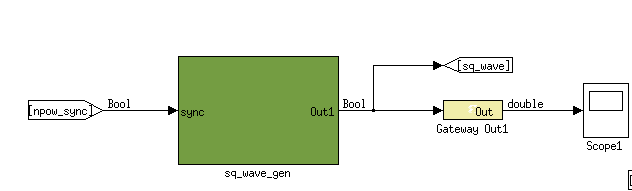
\includegraphics{sq_wave_gen_2.png}
\caption{The \textbf{sq\_wave\_gen} block generates a boolean signal which cycles between ON (True),
and OFF (False).}\end{figure}
\begin{figure}[htbp]
\centering
\capstart

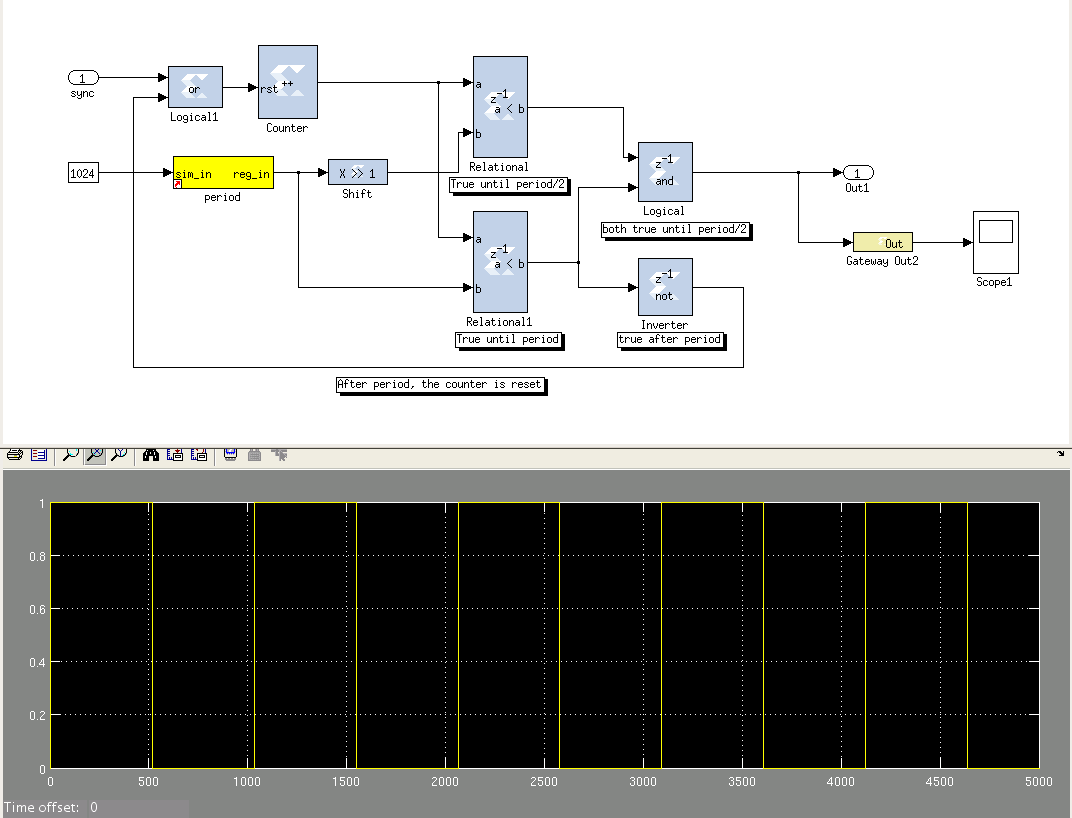
\includegraphics{sq_wave_gen.png}
\caption{The logic inside the \textbf{sq\_wave\_gen} block, and a simulated square wave.
This produces a boolean square wave signal of the given period.
The period can be controlled by the \textbf{period} register.}\end{figure}
\begin{figure}[htbp]
\centering
\capstart

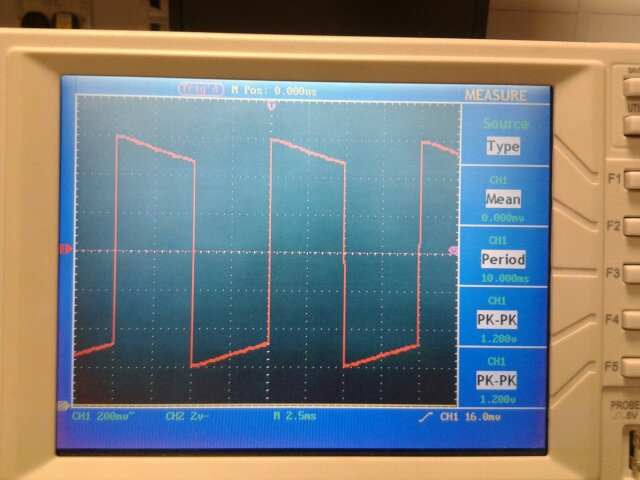
\includegraphics{nar_sq_wave.jpg}
\caption{The resulting square wave, as measured on an oscilloscope in the lab. The output of
\textbf{sq\_wave\_gen} is tied to the GPIO headers. These can run at up to 10 MHz, and output
a 3.3V level signal.}\end{figure}


\section{FFT and power}
\label{noise_diode:fft-and-power}
The output of the ADC is changed from 8\_7 bits to 18\_17 bits, then FFT'd.
There are 16 complex channels output. The power (autocorrelation) is taken,
then the signal is quantized down to 8 bits, in prep for the vector accumulator.
\begin{figure}[htbp]
\centering

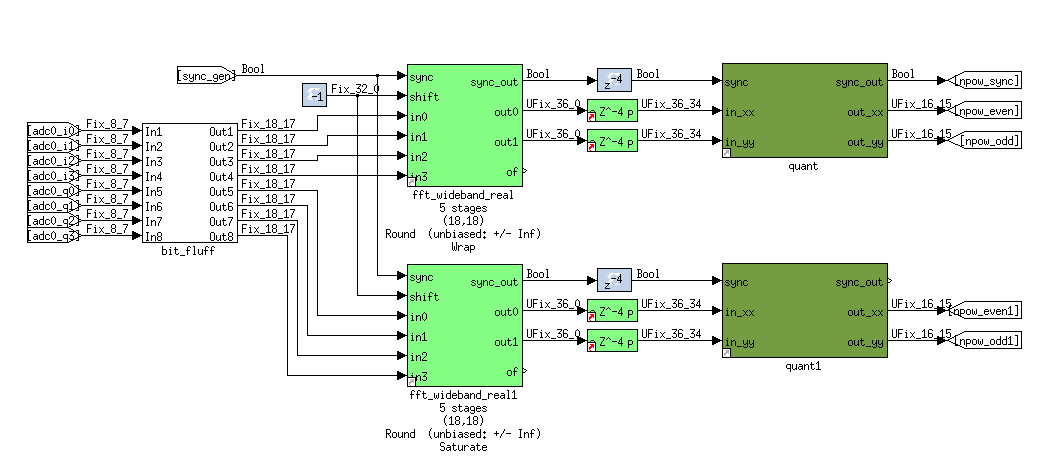
\includegraphics{fluff_fft_quant.png}
\end{figure}


\section{Demux and accumulation}
\label{noise_diode:demux-and-accumulation}
The output of the FFT needs to be separated into ON and OFF, which corresponds to the
noise diode being on and off. To do this, the square wave generator is used as an input
to a `demux' block.

After separating the two signals, they are fed into vector accumulators. As the vectors are
short (2x8 channels), bits grow quickly. As such, the input is 8 bit, and the output is 32 bit.
This gives 2\textasciicircum{}24 max accumulations before bit overflows can occur (might need to increase this).
\begin{figure}[htbp]
\centering

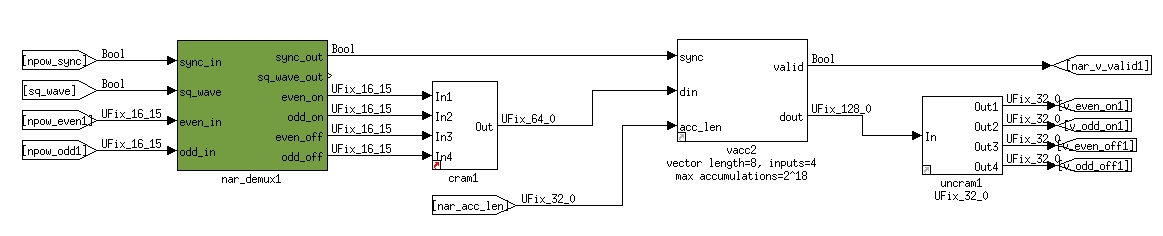
\includegraphics{demux_vacc.png}
\end{figure}


\section{Data readout}
\label{noise_diode:data-readout}
To compute the sum ON - OFF, the outputs of the vector accumulators are fed into an adder block
(which is set to minus). This creates a 33 bit signed number (can be -ve), which is recast to 32.

After this, the signal is buffered and then fed into a shared BRAM, which can be accessed via the
ROACH's Power PC.
\begin{figure}[htbp]
\centering

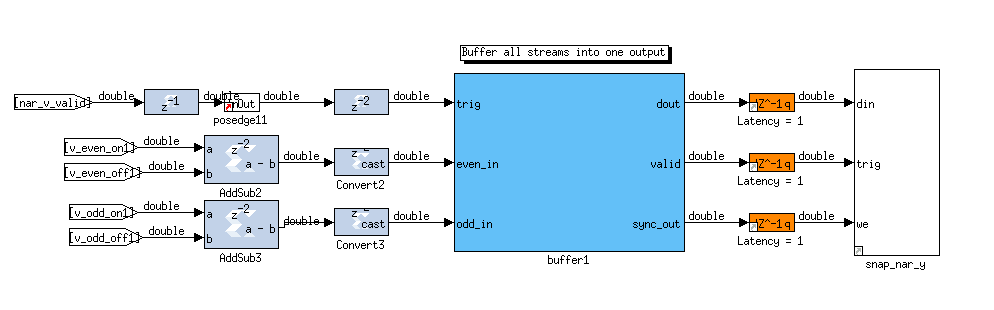
\includegraphics{buffer_snap.png}
\end{figure}


\section{Testing}
\label{noise_diode:testing}
TODO.


\chapter{Contacts}
\label{contacts::doc}\label{contacts:contacts}
\begin{tabulary}{\linewidth}{|L|L|L|}
\hline
\textbf{
Contact Name
} & \textbf{
Role
} & \textbf{
Email
}\\\hline

Danny Price
 & 
Project Manager
 & 
\href{mailto:danny.price@astro.ox.ac.uk}{danny.price@astro.ox.ac.uk}
\\\hline

Lister Staveley-Smith
 & 
Project Leader – Phase 1
 & \\\hline

Matthew Bailes
 & 
Project Leader – Phase 2
 & \\\hline

TBD
 & 
Project Engineer (software)
 & \\\hline

TBD
 & 
Project Engineer (hardware)
 & \\\hline

Erik Lensson
 & 
CSIRO coordinator
 & \\\hline

Douglas Bock
 & 
CSIRO coordinator
 & \\\hline

Brett Preisig
 & 
Parkes technical coordinator
 & \\\hline

George Hobbs
 & 
CSIRO Pulsar Scientist
 & \\\hline

Mike Jones
 & 
Oxford Coordinator
 & \\\hline

Matthew Bailes
 & 
Swinburne Coordinator
 & \\\hline

Robert Braun
 & 
Project CI: HI, noise cancellation
 & \\\hline

Steven Tingay
 & 
Project CI: Digital systems
 & \\\hline

Sascha Schediwy
 & 
Project Participant: System testing
 & \\\hline

Danny Price
 & 
Project Engineer: FPGA gateware
 & \\\hline

Willem Van Straten
 & 
Project Engineer: CPU/GPU
 & \\\hline

Jonathon Kocz
 & 
Project Engineer: PSR modes, RFI
 & \\\hline

Andrew Jameson
 & 
Project Engineer: GPU/GPU
 & \\\hline
\end{tabulary}



\chapter{Indices and tables}
\label{index:indices-and-tables}\begin{itemize}
\item {} 
\emph{genindex}

\item {} 
\emph{modindex}

\item {} 
\emph{search}

\end{itemize}
\begin{figure}[htbp]
\centering

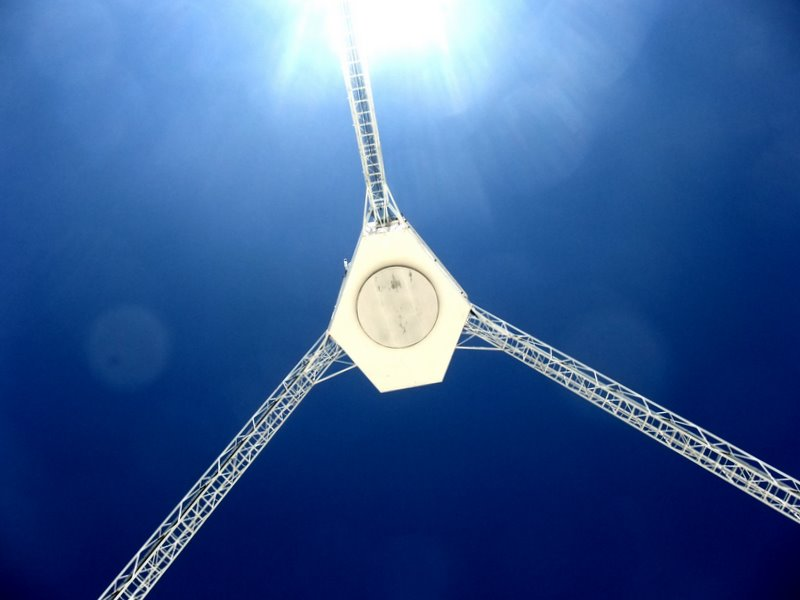
\includegraphics{parkes_focus.jpg}
\end{figure}


\renewcommand{\indexname}{Python Module Index}
\begin{theindex}
\def\bigletter#1{{\Large\sffamily#1}\nopagebreak\vspace{1mm}}
\bigletter{h}
\item {\texttt{hipsr\_gui}}, \pageref{software:module-hipsr_gui}
\item {\texttt{hipsr\_server}}, \pageref{software:module-hipsr_server}
\end{theindex}
\renewcommand{\indexname}{Python Module Index}
\begin{theindex}
\def\bigletter#1{{\Large\sffamily#1}\nopagebreak\vspace{1mm}}
\bigletter{h}
\item {\texttt{hipsr\_gui}}, \pageref{software:module-hipsr_gui}
\item {\texttt{hipsr\_server}}, \pageref{software:module-hipsr_server}
\end{theindex}

\renewcommand{\indexname}{Index}
\printindex
\end{document}
